\documentclass[a4paper]{report}

\usepackage[masterthesis,english]{comp}
\usepackage{graphicx}
\usepackage{hyperref}
\usepackage{multirow}
\usepackage{mathtools}

\title{A General Aspect Orientation Framework}
\author{Chris Vesters}
\principaladviser{Dirk Janssens}
\assistantadviser{Tim Molderez}
\submitdate{May 2014}
\bibfile{references}
\bibpunct{[}{]}{;}{a}{,}{,}

% Make hyperref package use black links
\hypersetup{
	pdfauthor={Chris Vesters},
	pdftitle={A General Aspect Orientation Framework},
	pdfkeywords={Aspect Orientation, Framework},
    colorlinks,
    citecolor=black,
    filecolor=black,
    linkcolor=black,
    urlcolor=black
}

\begin{document}
\frontpages

\clearpage 
\phantomsection 
\addcontentsline{toc}{chapter}{Nederlandstalige Samenvatting}
\chapter*{Nederlandstalige Samenvatting}

\clearpage 
\phantomsection 
\addcontentsline{toc}{chapter}{Acknowledgements}
\chapter*{Acknowledgements}

\clearpage 
\phantomsection 
\addcontentsline{toc}{chapter}{Abstract}
\chapter*{Abstract}

\mainbodypages

\chapter{Introduction}
\section{Aspect Oriented Programming}
Aspect oriented programming (from now on referred to as AOP) is a way of programming that allows separating code beyond the capabilities of object oriented programming. It allows the separation of cross cutting concerns from the core concerns, by doing this we achieve more modular code, prevent code tangling and code scattering which results in code that is easier to maintain and modify.
\begin{figure}[h!]
\centering
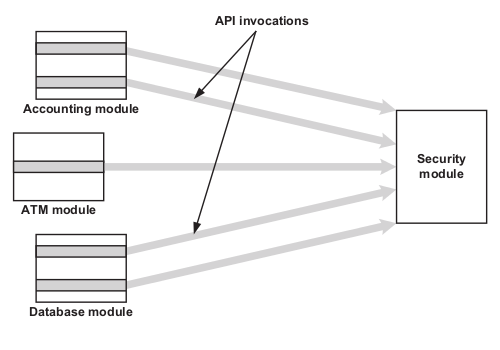
\includegraphics[scale=0.5]{images/Code_Scattering.png}
\label{fig:Code_Scattering}
\caption{A representation of code scattering\cite{Laddad10}.}
\end{figure}\\
\begin{figure}[h!]
\centering
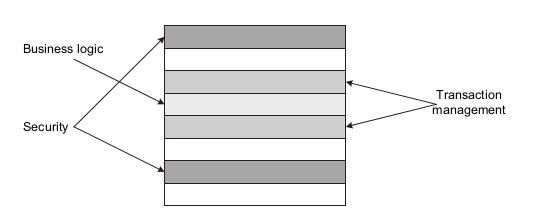
\includegraphics[scale=0.5]{images/Code_Tangling.png}
\label{fig:Code_Tangling}
\caption{A representation of code tangling\cite{Laddad10}.}
\end{figure}\\
AOP works by identifying join points, which is certain point in the execution of the program. The set of all the join points is called the join point model. It is at these join points that we can modify the original program execution. This change can go from something as simple as logging to something more invasive where the original code isn't even executed at all.\\
A first thing we need is a way to indicate which join points we want to work on, this is done by a point cut. Now we can refer to certain join points we also need a way to modify the execution. This is done by an advice, note that there can be multiple kinds of advice.\\
In the end everything has to come together, this is done by the weaver.\\
\\
The most known AOP language by far is AspectJ, which is an extension of Java. To demonstrate the concept of AOP a couple of AspectJ examples are shown here:\\
TODO: EXAMPLES!\\

\section{Problem}
Currently AOP is often implemented by extending an existing language, this often leads to completely new languages requiring new compilers and  breaking existing tools for the base language. Especially the latter is a reason why some people haven't made the step to start working with aspect oriented languages.\\
\\
Though the concepts of AOP are quite general, which is reflected by the similarities in different aspect oriented languages, all the AOP parts of these languages were written from scratch. The main reason for this is the absence of a general language independent library or framework to handle aspect orientation. Another reasons is that by building a language from scratch you get more freedom to implement the desired features.

\section{Goal}
The goal of this thesis is to build a framework that encloses all core ideas of AOP in an abstract manner without being specific about a particular base language. This will enable use to use the framework to develop an aspect oriented language quicker and easier than currently is the case by extending a couple of parts. The framework will work for completely new languages, and existing ones we want to extend. The latter one will pose the most problems as the freedom to adapt the compiler is very limited. (TODO: add in a later section the idea of injecting the code into a compiler with AspectJ)

\chapter{Aspect Oriented Language Components}
An aspect oriented language consists of several components, to explain these I will start from the base language and work my way up to get an aspect oriented language. At every point I'll make it more concrete with a small AspectJ example.\\
\\
The starting point of creating an aspect oriented language is the base language, this is the language that we want to extend or is a completely new language. In the latter case the base language will be the new language excluding all the aspect oriented features. The base language can be any kind of language: procedural, object oriented, functional, logical, data oriented, ... (TODO: EXAMPLE)\\
\\
By defining the base language we implicitly defined a join point model. This is because the join point model consists of all the points that occur during execution on which intervention of the aspects is allowed. The join point model will always remain implicit, but it is an important part of any aspect oriented language as it is the link between the base language and the aspect oriented part.\\
\\
Knowing at which points we can intervene doesn't allow us to do anything, we need a way to identify certain points. This identification is done by using pointcuts, specifying one or more join points. They way in which pointcuts allow us to refer to join points should be as close as possible as the way in which they appear in the base language. (TODO: EXAMPLE)\\
\\
Now that we can refer to certain join points, we can actually start modifying the original code. This modification is encapsulated in an advice, which contains 'code' that has to be executed. When this 'code' is executed is defined by the pointcut with which the advice is associated. Whenever the program passes a join point that matches with the associated pointcut, this advice must be executed. The 'code' in the advice should be written in the base language to prevent the user from learning an entire new language. (TODO: EXAMPLE) The advice should also be able to have access to information about the join point, this information will be provided by the pointcut.\\
\\
One problem that arises is: what is suppose to happen if we encounter a join point at which multiple advices are to be executed? This can be either caused by multiple pointcuts matching to the join point, or multiple advices being associated with the same pointcut. The latter case can be easily solved as we can combine the two advices into one bigger advice. The first is a bit more tricky since the one pointcut can also match other join points, different from the other, which means we can't just combine them. (TODO: illustrate) The solution to this is of course to introduce an ordering mechanism. This ordering can be either placed on the pointcuts or on the advices, in the first case we still need to make sure that there is only one advice for each pointcut though.\\
\\
One final component we need, is something that will actually make sure that the advices are executed when the join points are encountered. The weaver will make this happen, and can do this in multiple ways. The easiest is compile-time, weaving which comes down to a pre-processing step, a more advanced form is run-time weaving, yet other forms are available depending on the base language. (TODO: EXAMPLE)\\
\\
With the components specified above we are perfectly possible to create an aspect oriented language, despite that we note that some features are still missing, as an example we note that communication between different advices is impossible. Since aspect orientation is often presented as an extension of object oriented programming it makes sense to introduce some form of class, called aspects. These aspects will contain the advices, which match functions and methods in object oriented languages, and can be extended to have members too. By doing this we immediately have can provide the advantages offered by object oriented languages among which are inheritance and encapsulation. (TODO: EXAMPLE)\\
\\
An overview of all the components and how they are linked together is shown in figure (TODO:REF). The weaver is not considered to be part of the aspect language just as a compiler is not considered a part of the language.

\chapter{Aspect Oriented Framework}
Since the framework has the be easily extensible to work with any kind of language it has to be very abstract and may not contain any information about a base language. On the other hand, creating a framework that is too abstract and general requires too many additions to be made to implement it for a base language, making the framework completely missing its goal. The level of abstraction has to be well considered.\\
\\
I will first go into detail how the components that were identified in the previous chapter are represented and work in the framework. The explanation of the weaver is preceded by some information that is required to fully understand how the weaver works. This is followed by some remarks about the current version of the framework, and to conclude the chapter I explain how we can now expand this framework to work with any base language.\\
\\
The first component of the aspect language that we identified were the pointcuts. This component is implemented as an abstract class Pointcut, to completely specify a join point we need some way to identify it's signature, this however is language specific and can therefore not be provided by the framework. Other common structures are arguments and context. The arguments are meant for information that can be used in the advice, while the context is a way to restrict matching join points based on  information that goes beyond the scope of the join point.\\
\\
Something we notice, which is also the case for AspectJ, is that it is not possible to identify completely different join points with one pointcut. This complicates writing advice that has to be executed on these two different sets of join points. To simplify this we allow grouping pointcuts into sets, this is implemented as a PointcutSet, which has a set of pointcuts, arguments that are available for the advice, and should be present in all the poincuts of the set, and a name so we can link the advice to this pointcut. (TODO:REF)
\begin{figure}[h!]
\centering
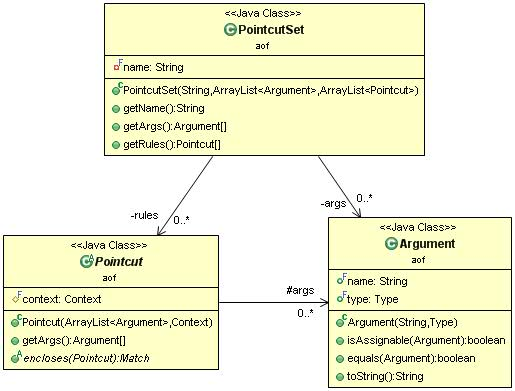
\includegraphics[scale=0.7]{images/AOF/PointcutSet.jpg}
\label{fig:PointcutSet}
\caption{UML diagram of the PointcutSet and Pointcut.}
\end{figure}\\
\\
The advices are implemented by the abstract Advice class. This class has a name, which will make ordering them a lot easier, and a set of arguments, these arguments are the ones that can be used inside the advice body. Note that the arguments of the pointcut to which this advice is linked must be assignable to these arguments. The body or actual code of the advice is not provided by this class, simply because it depends on the base language as we want this to be in the same formalism. (TODO: ADD REFF)
\begin{figure}[h!]
\centering
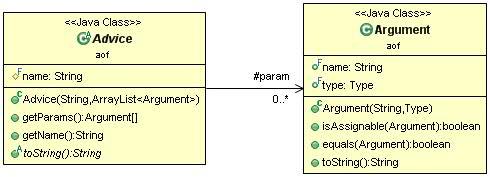
\includegraphics[scale=0.7]{images/AOF/Advice.jpg}
\label{fig:Advice}
\caption{UML diagram of the Advice.}
\end{figure}\\
\\
Before going any further some more explanation about some already mentioned concepts is required. I have talked about arguments and a context, but didn't mention what these are. An argument is a hard to abstract as every base language has its own vision of what an argument is, though two concepts are very common, being a name and a type. For this reason the Argument class has a name, which is also required for access to the argument and a type. The type however can not be a base language type, but should be more general. For this reason an interface called Type was created. A context is easier, since  the context can be anything and highly depends on the base language the only thing the framework provides is an interface Context. Note that the Context and Type interface are exactly the same, I will discuss this into more detail in chapter (TODO: REF DISCUSSIONS). (TODO: ADD REFF)
\begin{figure}[h!]
\centering
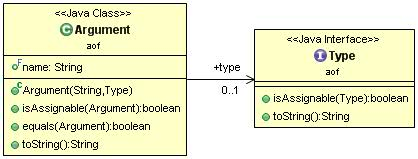
\includegraphics[scale=0.7]{images/AOF/Argument.jpg}
\label{fig:Argument}
\caption{UML diagram of the Argument class.}
\end{figure}\\
\begin{figure}[h!]
\centering
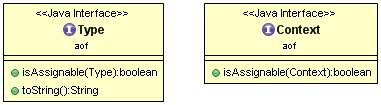
\includegraphics[scale=0.7]{images/AOF/Type-Context.jpg}
\label{fig:Type-Context}
\caption{UML diagram of the Type and Context interface.}
\end{figure}\\
\\
This being said we can now discuss the remaining components being: the order mechanism, the aspect and the weaver. The components will be handled in the order they are specified here.\\
\\
The framework does not provide a basis for the ordering. This means that the user is free to implement the way of specifying an ordering as he likes. The user is also free to choose whether the order will be specified on the pointcuts or on the advice. Despite the freedom on the ordering 'language' the ordering itself is still limited. This will be discussed into more detail once the weaver is introduced.\\
\\
The current version of the framework does not provide any concept of 'aspects', though this causes some limitations, it does not make the framework useless. Some of the limitations were already mentioned in the previous chapter, more details about the consequences of the absence of an encapsulating aspect is discussed at the end of this chapter.\\
\\
Before discussing the weaver we have to make some things a bit clearer. You might be wondering how the join points will be extracted from the source code. This is done by the parser of the base language, or a modification of it. The join points that are generated by this parser will actually be instances of the Pointcut class. By doing this comparing whether a pointcut set contains a pointcut that matches the joinpoint becomes trivial.\\
\\
Something you might have noticed is that the advice does not keep a link to the pointcut itself, nor the other way around. The link between pointcut and advices is handled by the weaver, this allows a better separation between pointcuts and advices and gives the weaver more freedom to operate.\\
\\
The ordering mechanism requires some extra information as well, I mentioned earlier that despite the freedom some limitations still exist. This is cause by the way the weaver handles the ordering internally. The weaver will keep a list for every advice to its preceding advices. This means that the ordering provided to the weaver has to be on the advices, and should result in a partial ordering (TODO: add image)\\
\\
A final remark that has to be made is how the framework handles the argument mapping from adivce to pointcut and join point. For this the framework provides a Match class that contains a dynamic value for each argument. (TODO: add REFF) We can use this match to get the join point specific value for an argument of the advice.
\begin{figure}[h!]
\centering
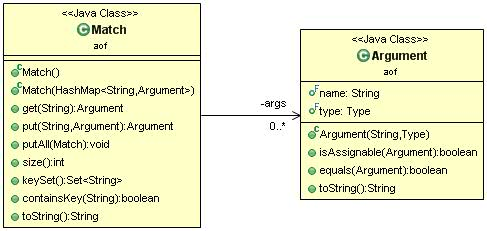
\includegraphics[scale=0.7]{images/AOF/Match.jpg}
\label{fig:Match}
\caption{UML diagram of the Match class.}
\end{figure}\\
\\
This brings us to the last component, the weaver. Just like most elements in the framework is the weaver implemented as an abstract class. This abstract class provides a way for all components to register their information, which is then stored to be processed. They way in which the information can be processed depends both on the base language and the possibilities of the base language parser and can therefor not be implemented by the framework. The framework does however provide a way to specify the input and output files by using flags, an overview of these flags can be seen in (TODO:REF).
\begin{table}[h]
\centering
\begin{tabular}{l l}
-a \textit{files} & Specify the aspect files.\\ [2ex]
-s \textit{files} & Specify the source files.\\ [2ex]
-oDir \textit{dir} & Specify an output directory (optionally).\\
\end{tabular}
\caption[tab:Flags]{An overview of the flags available in the weaver.}
\label{tab:Flags}
\end{table}\\
Besides that it also provides some methods that simplify processing the information. The most important one is 'executingAdvices', given a certain joinpoint this method will return all the advices that have to be executed in the order they are returned. In case the user needs to know the pointcuts that match a certain joinpoint a method 'enclosingPointcuts' is provided. The framework also implements a way to compare advices based on the partial ordering, this is done by the AdviceComparator which is an extension of the Comparator. This is meant for internal usage and the user should not need to use this since the return value of the 'executingAdvices' method is already ordered. (TODO: add REF)
\begin{figure}[h!]
\centering
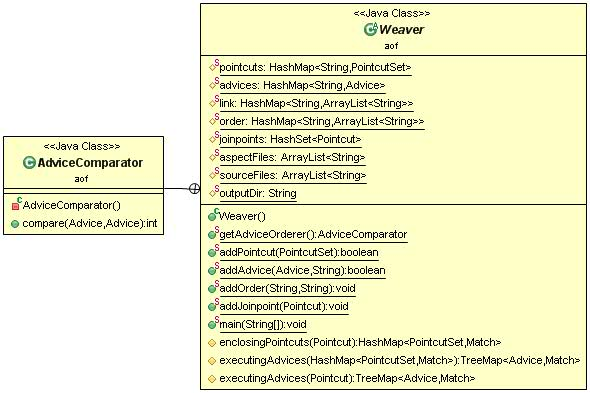
\includegraphics[scale=0.7]{images/AOF/Weaver.jpg}
\caption{UML diagram of the Weaver class.}
\label{fig:Weaver}
\end{figure}\\
\\
A complete overview of the framework and how everything is connected can be seen in figure (TODO: REF).
\begin{figure}
\centering
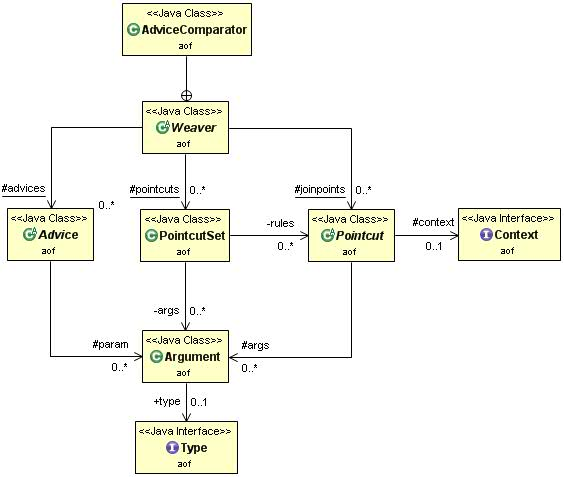
\includegraphics[scale=0.65]{images/AOF/Full.jpg}
\caption{UML diagram of the entire framework.}
\label{fig:FullView}
\end{figure}
\\
TODO: some remarks about this?\\
\\
Some trade offs had to be made when designing the framework, it are these trade off that I now discuss into more detail. First of all it needs to be noted that both Context and Type are interfaces which both specify only one method called 'isAssignable'. This means that Context and Type, though called different, do the same thing. We could use one general interface, this is not done though to be able to handle future evolution.\\
\\
Adding a notion of aspect would allow a lot of nice features such as adding members that can be used for communication between advice and inheritance. They could also be used as a way to encapsulate pointcuts and advice, though this can also be done without aspects simply by separating them over multiple files.\\
Adding aspects to the framework would have introduced a lot of extra complexity. Since the goal of this thesis is to demonstrate the usability of such a framework I have chosen to not include this, but keep it as a future work.\\
\\
The framework uses an abstract notion of type, this is to achieve the level abstraction required to separate the framework from the base language. This however means that for each base language we need a new type system that implements the Type interface, which might result in a lot of work. Sometimes it is however possible to use the same type system the compiler of the base language uses if we can add the interface to it.\\
\\
The advice and pointcuts are not directly connected with each other, the connection is achieved by the weaver. Because adding an explicit link does not provide any advantages, I have chosen to do it this way to ensure that the components are as loosely coupled as possible. Nevertheless the framework demands that at the moment a pointcut is added the pointcut set it is linked with must be be known to the compiler.\\
\\
Something that was not discussed so far is what happens if a join point is encountered that is matched by multiple pointcuts in the same pointcut set. In this case there basically are two options: either we execute the advices for each matched pointcut, or we only select the first matched pointcut of the set. Currently the latter is implemented in the framework, mostly because if we still want the first to happen, we can simply split the pointcut set.\\
\\
One final remark that has to be made is that implementing both join points and poincuts as the same Class can be dangerous since they are not the same. One example is that poincuts can contain wildcards wile join points should not. It may also be feasible to allow specifying types and sub-types in pointcuts, where in the join point the types are fixed and known. This means that we have to use the Poincut class carefully if we use it with a join point.\\
\\
(TODO: can we ommit the context type and just add all this stuff as arguments?)\\
\\
To conclude this chapter I will briefly explain how the framework can be expanded to work with a base language, for more detailed examples I refer to chapters (TODO: REF) where the framework is expanded for two different languages. Before being able to use the framework you have to specify a language in which it is possible to specify pointcuts, advice and optionally an order. You have to provide a parser for this language, which will create the pointcuts and advices which are handed over to the weaver. Due to the separation of the components it is possible to have separate languages for the pointcuts, advice and order, each with its own parser. In practice this will not be such an attractive option though since it involves a lot of extra work.\\
\\
The pointcuts and advice that has to be created has to be specific for the base language, this means that you first have to create a subclass of Advice and one or more subclasses for Pointcut.
The advice subclass is simple, it must contain the body of the advice. The pointcuts need to contain all information to identify a join point. Since there will be multiple types of pointcuts you will have to implement one subclass for each type of pointcut. If you desire to add a context to the pointcut, you still have to create a class with the Context interface that contains all the context information you want to use.\\
\\
The pointcuts and advices of course require you to implement a type system. Depending on the availability of the type system used by the base language, and more precise the compiler, it is possible to add small modifications to get the type system without much work. If not, this might be a bigger problem.\\
\\
Now you can create pointcuts and advice you still need to expand the Weaver class to add the actual weaving. Since the framework gives you the advices to execute for each join point all the extended weaver has to do is execute these advices at those times. This sounds easier than it sometimes is though, especially the way of how you can interact with the base language is important. (TODO: overview of interaction between languages and weaver)\\
\\
I know this sounds vague and very abstract, which is why I refer to chapters (REF) again since they contain worked out examples.

\chapter{Small C}
Small C is a subset of the C language, which makes it an procedural language. Though it does not support structs or including other files, it does give us a good overview of what aspect orientation in a procedural programming language is like. Besides this, the presences of a modifiable compiler made this language an interesting first step to test the framework.\\
\\
Despite the resemblance with C, I specify some examples to show the normal structure of a Small C program.\\
\\
TODO: EXAMPLE OF SMALL C

\section{Join Point Model}
Due to the minimalistic character of the language the join point model is limited too. The join points identified can be divided into two groups, each with two types. An overview of the join points is given in table (TODO: REF).
\begin{table}
\centering
\begin{tabular}{|l|l|l|}
\hline
Join Point & Type & Description\\
\hline
\multirow{2}{*}{Function} & Call & The moment a function is called.\\
& Execution & The moment a function is executed\\
\hline
\multirow{2}{*}{Global Variable} & Set & The moment a global variable is set.\\
& Get & The moment a global variable is accessed.\\
\hline
\end{tabular}
\label{tab:SmallC_JoinPoints}
\caption{Small C join points.}
\end{table}

\section{Base Language Compiler}
TODO: explain how the base language compiler was used to get the joinpoint.

\section{Aspect Language}
Before discussing the parts of the framework it is required to explain some basic elements of the language. Though the language is mostly based on AspectJ, there are some differences mostly caused by the attempt to keep the language as simple as possible.\\
\\
Since we don't want to specify each member or method explicitly, the concept of wildcards is often introduced. This is also the case for this language, the '..' wildcard allows the user to specify a space that can be covered by any 0 or more characters.\\
\\
The compiler I used already had an entire type system, which could easily be used for the framework too. (TODO: REFF) To support wildcards an extra type, the AnyType, was added. This type will allow the user to leave the type unspecified. Note that it is impossible to partly specify a type such as '..int' which could match types such as longint, shortint and int. This is not a problem since the only types allowed in Small C are: 'int', 'float', 'char', 'void' and 'boolean' in combination with the array and pointer additions.\\
\begin{figure}
\centering
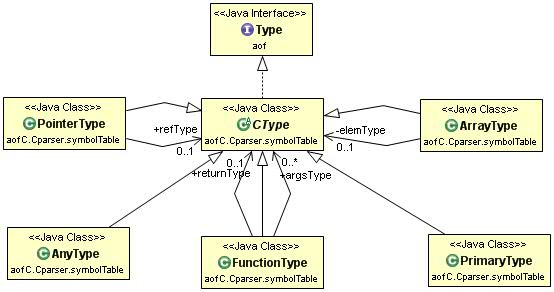
\includegraphics[scale=0.7]{images/AOFC/CType.jpg}
\caption{UML diagram of the CType class and its subclesses.}
\label{fig:CType}
\end{figure}
\\
A complete overview of the language in a visual BNF form can be seen in figure (TODO: Add diagram). Keep in mind that the explanation of most parts is still to come.\\


\section{Pointcuts}
The join points are mapped to pointcuts in a one-on-one manner. For each join point there exists a pointcut, being MethodPointcut and MemberPointcut. The different types are handled by adding a flag to the pointcut to indicate the type. Because identifying a method or a global variable is totally different we need to separate these two. But because a call and an execution both execute on a method we can combine these two together. This also holds for the get and set of a global variable.\\
\\
To identify a method join point we need the signature of the method, consisting of the name of the method, the return type and a set of arguments. Note that the arguments are already implemented by the abstract super class, and thus are not part of the MethodPointcut class. (TODO: REFF). Note that wildcards can be used in every element of the pointcut: in the name of the method, as a type of an argument, as  return type or as part of the argument list. It is not allowed to use a wildcard in the name of the arguments since these will be passed on to the advice to be used there, doing this wouldn't make any difference because the arguments are only matched on type and not on name. The names however are used to map them onto the arguments specified in the pointcutset. It is therefor also required that a pointcut contains all the arguments the ecnlosing pointcutset does. (TODO: add examples).\\
\begin{figure}
\centering
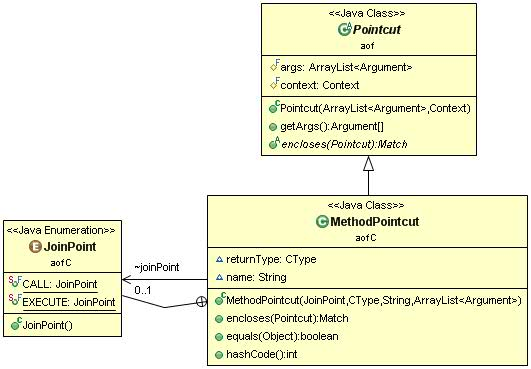
\includegraphics[scale=0.7]{images/AOFC/MethodPointcut.jpg}
\caption{UML diagram of the MethodPointcut class.}
\label{fig:MethodPointcut}
\end{figure}
\\
The MemberPointcut is pretty empty, simply because the best way to identify a global variable is to see it as an argument of the pointcut. By doing this the only thing the MemberPointcut class has to add is the flag to identify the different types. (TODO: REFF) Just as with the MethodPointcut it possible to use a wildcard as type, but it is also allowed to specify a wildcard as (part of) the name of the member to match multiple global variables. Because a MemberPointcut only contains one argument, being the member, it is always this argument that is mapped to the pointcutset arguments. (TODO: add examples)\\
\begin{figure}
\centering
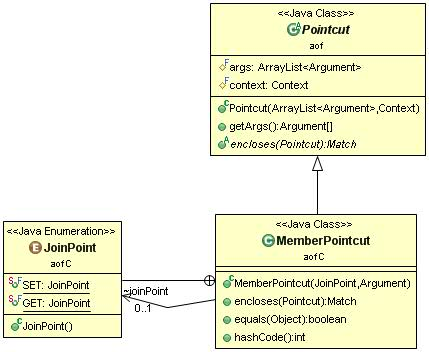
\includegraphics[scale=0.7]{images/AOFC/MemberPointcut.jpg}
\caption{UML diagram of the MemberPointcut class.}
\label{fig:MemberPointcut}
\end{figure}
\\
The current implementation does not use the context of the framework, which limits usability. Yet I am convinced that adding a context would not add much functionality since the only context in Small C is the call hierarchy. Note that due to the lack of a context in the pointcuts the method call and execution pointcut will yield the same result, with a context we could for instance get the current method.

\section{Advice}
The advice of our aspect oriented version of Small C is very basic, it contains a string which represents Small C code. The code is allowed to contain arguments that are defined by the pointcutset it is linked to, but these are not treated specially in the CAdvice class itself (TODO: REFF). Besides the code, the CAdvice class also contains some timing information. This breaks the clear separation between pointcuts and advice and can be considered to be bad programming, yet this way we can create pointcutsets that are more re-usable. The different types, specifying the moment of execution, are before, after and around. These are the same as are present in AspectJ, and are pretty straightforward. Only the around advice may need some more explanation. (TODO: give the explanation) (TODO: explain the different types of advice)\\
\begin{figure}
\centering
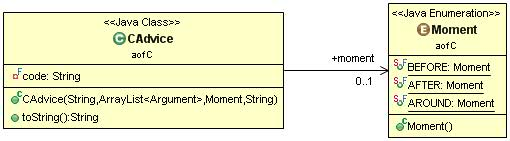
\includegraphics[scale=0.7]{images/AOFC/CAdvice.jpg}
\caption{UML diagram of the CAdvice class.}
\label{fig:CAdvice}
\end{figure}
\\
An advice needs to be linked with a pointcutset, this is done by referring to it's name and specifying the arguments it requires. Note that the arguments need to match on type, but may differ on name, the names used in the advice can be used in the body of the advice.\\
\\
The body of the advice is not parsed in any way, at the moment it is created. It is not even parsed anywhere in the entire process until the very end which is simply compiling the weaved code. (TODO: add examples)

\section{Order}
There are two situations in which multiple advices can be mapped to the same moment in execution. The most obvious situation is when multiple advices are linked to the same pointcut set, but also if we have multiple pointcutsets that happen to match the same join point. In both cases it is possible that advices give rise to conflicts, but only if their types overlap.\\
\\
First of all we will discuss the natural order of the advices. If there is no conflict the order is determined by the type of the advice (TODO: add image an overview of the different types of advice and their order), if there is a conflict but no order, it's up to the framework to resolve it.\\
\\
To determine the order when conflicts do arise it is possible to specify an order between any two advices, even those that can never cause a conflict which may seem useless. However, it becomes useful in the case where you want more than two advice to be in a specific order and they are of different types. (TODO: add example of before, after and arround with order).
(TODO: add examples)

\section{Weaver}
The weaver is the biggest piece of code, after all it is the core part of every aspect oriented language. Once it has all the information it can start putting it together, it does this by writing wrapper methods for the join points, even if there is no advice to be execute for this join point. This last could have been omitted, but for simplicity it is not. Which wrappers are generated depends on the join point, and partly on the advices. For every global variable declared there will be two wrappers, one to handle the access to the variable, and another for the assignment of a new value. (TODO: add example) The same holds for a method but with call and execution instead. (TODO: add example) The original operations will be modified so that they use the wrappers instead. (TODO: add examples)\\
\\
Besides these wrappers some other methods are generated as well. One for each advice of the type before or after, and one for each matching join point of an around advice. The reason the around advices needs multiple instances is that it will have to proceed to the original method. While this is not the case for the before and after advice, it is still much easier to put them in a separate method, especially if you consider that such an advice can alter the values of arguments, but that these changes may not be passed on to the actual method, only the around advice may do such things. (TODO: add examples)\\
\\
Besides generating wrappers, the weaver is also responsible for delivering the right arguments to the advice, this is another situation that shows the advantages of putting an advice in a separate method. The around advice also contains a proceed() call, the weaver has to replace this with a call to the original method or next around advice. The arguments specified in the proceed must be conserved and passed on. To not complicate the weaver any further it is required that the user manages the declaration of a value to store the return result and explicitly returns this value if a return value is required. The declaration, assigning the return value of the proceed() and return the value all must occur separately. This is because it is possible that the weaver will insert calls to other advices before and after the proceed call. (TODO: add examples).\\
\begin{figure}
\centering
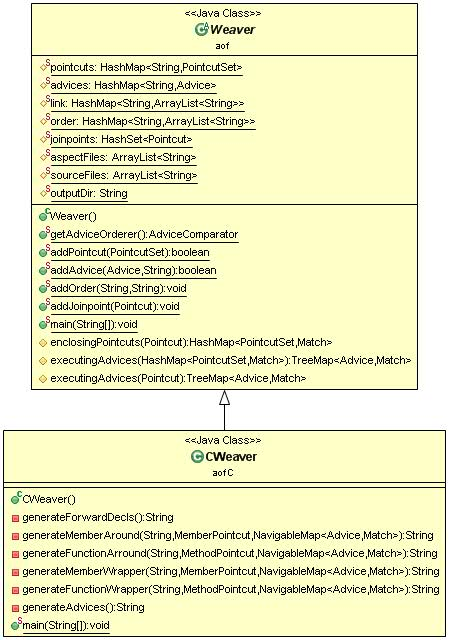
\includegraphics[scale=0.7]{images/AOFC/CWeaver.jpg}
\caption{UML diagram of the CWeaver class.}
\label{fig:CWeaver}
\end{figure}
\\
Now that all the components have been introduced, I give a final overview of the entire structure to make it extra clear how all the components are connected.\\
\begin{figure}
\centering
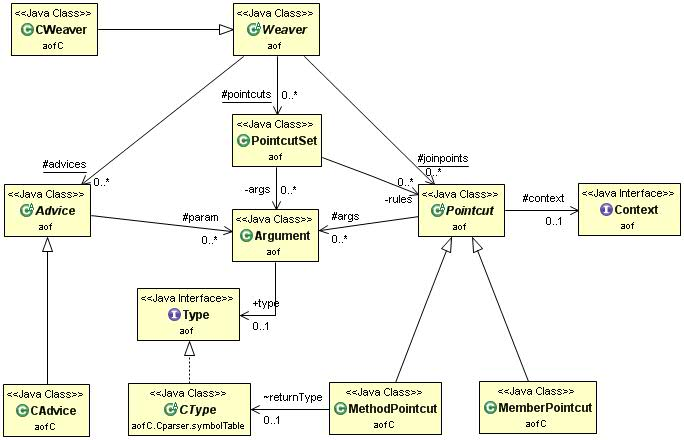
\includegraphics[scale=0.55]{images/AOFC/CFull.jpg}
\caption{A full overview of the use of the framework for Small C.}
\label{fig:CFull}
\end{figure}

\section{Examples}
TODO

\section{Difficulties}
Despite having a modifiable compiler, there were a lot of problems of weaving the advices into the code. This was caused by the fact that the compiler was not designed to allow changes after parsing the code. Changing this would require big changes in the compiler and was therefor not really an option. Instead of changing the compiler another alternative was used, by creating two compilers, both with small changes, we could weave the file in multiple passes.\\
\\
In phase 1 the source code will be parsed and all join points will be specified to the weaver. The weaver will produce wrappers and add these to a temporary output file. In phase 2 the modified file will be parsed and the original calls will be modified to point to the wrappers. In phase 3 the actual advice bodies will be written to the wrappers. Phase 4 is to compile the weaved file with a regular compiler, this is not done by the weaver and has to be done by the user himself.\\
\\
It was impossible to change the calls in the first phase due to a simple circular dependency. The compiler checks that the called function actually exists. Since the compiler does not allow to add declarations before the current point, these declarations have to exist in the source code itself. To do this however we need to know which join points occur, and thus we need to have parsed the file before.\\
\\
Adding the content can not be done before phase 2, simply because the content contains function calls to the actual functions which need to be kept. It is impossible to distinguish a call from within a wrapper from one within a 'normal' function, yet we need to treat them separately. Therefor we need to add the content in a separate phase.

\chapter{Dot}
Dot is a language that allows you to easily specifies the structure and appearance of a graph. Some of the features the language supports  are directed edges, undirected edges, subgraphs, labels for nodes and edges, different shapes, colors and more. Despite that it is a pretty simple to use language, and has a very straightforward syntax it tends to be very verbose when trying to create large and complicated graphs.\\
\\
Dot does not have any time related aspect as the result of the 'compiler' is the graph that the user wants. Because of this it adding AOP may seem weird since join points are defined as points in the execution of a program. Since the program does not execute, but is a static graph, all the join points simply map to points in the code in a static way. Yet the ideas of AOP can still be applied.\\
\\
Because the syntax of Dot is that self-explaining, showing a few examples is enough to get an understanding of the language.\\
\\
TODO: EXAMPLE OF DOT

\section{Join Point Model}
The join points identified in Dot are all the elements of the graph, being the graph itself, nodes and edges. This simple join point model is mostly caused by the lack of run-time behavior.

\section{Base Language Compiler}
TODO: Explain the base language compiler. This was a very simple to modify compiler, that's about all I remember.

\section{Aspect Language}
The aspect language mostly uses the same syntax as Dot itself to keep the language as simple as possible. There exists a wildcard to create more general rules, being '..'. By using this the programmer specifies that anything can take its place.\\
\\
TODO: explain the concept of Attributes: how is this used?
TODO: explain the type system.\\
\begin{figure}
\centering
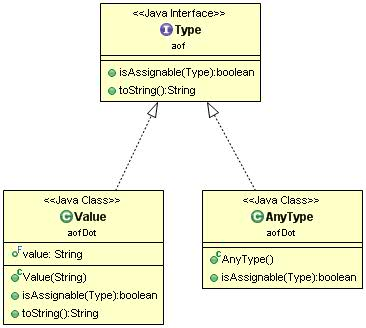
\includegraphics[scale=0.7]{images/AOFDot/DotType.jpg}
\caption{UML diagram of the type system for aspect orientation in Dot.}
\label{fig:DotType}
\end{figure}

A complete overview of the language in a visual BNF form can be seen in figure (TODO: ADD DIAGRAM).

\section{Pointcuts}
Every join point is expressed by a pointcut, resulting in three pointcuts being GraphPointcut, NodePointcut and EdgePointcut which represent respectively a graph, node and edge. All of these pointcuts can have Dot attributes, these will be stored as arguments and thus are part of the superclass Pointcut. But because each pointcut also has specific information I will now discuss these three pointcuts into more detail.\\
\\
The GraphPointcut requires all the information of it's nodes and edges. Instead of introducing new types for nodes and edges, it is easier to reuse the pointcuts to represent this. A graph also has a name, though this information is not used in the current version.\\
Checking whether a graph matches with a GraphPointcut is very simple, we just need to compare the nodes and edges it contains, which is discussed when we introduce these pointcuts and we need to verify that all the attributes are present and have the same value if any specified. A wildcard can be used to indicated that the graph may contain more nodes and edges, or that the attributes is just a subset.\\
TODO: Example\\
\\
A NodePointcut is the easiest as it only has a name and attributes, and since attributes are already handled by the superclass all we need to do is add a name. A node matches a NodePointcut if it has the same name and all the attributes match.\\
TODO: Example\\
\\
An EdgePointcut isn't that much harder, thanks to the compiler every edge contains exactly two nodes: a source and a target. These two nodes are again represented by a NodePointcut, as this was the easiest solution. On top of that we also need to know whether the edge is directed or not, which is a simple boolean. An edge matches a pointcut if they are either both directed and the sources and targets match, if they are both undirected the source and target node may be switched. (TODO: check this: may be an error in the current version!).\\
TODO: Example\\
\begin{figure}
\centering
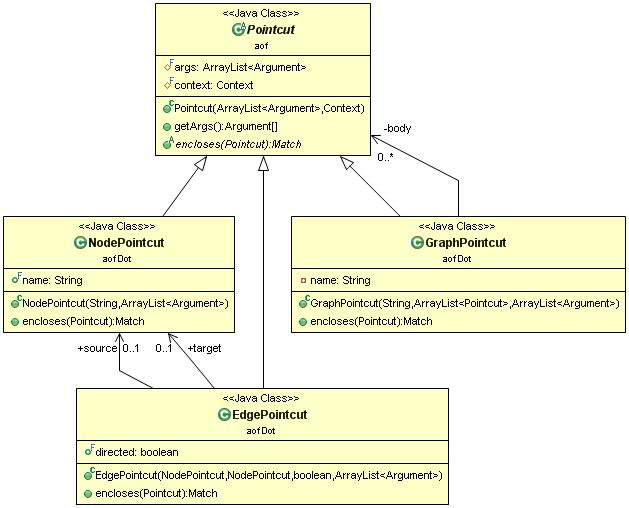
\includegraphics[scale=0.3]{images/AOFDot/DotPointcuts.jpg}
\caption{UML diagram of the three pointcut classes.}
\label{fig:DotPointcuts}
\end{figure}
\\
The current version does not use the context mechanism, but the user can specify that a form of context by wrapping it in a graph. By doing this, we can make a link between different elements in the same graph. I believe that this is also the only possible use for a context in Dot.\\
\\
Parameters can be introduced on every level of the pointcut, this means that we can specify a GraphPointcut but introduce a parameter for one of it's NodePointcuts.\\
TODO: Example

\section{Advice}
There exists two kinds of advice: insert and delete, which are meant to respectively insert elements or delete them from the pointcut. To provide this functionality the DotAdvice is created, this contains the type of the advice and the body, being the elements that have to be inserted or deleted. These elements are expressed using the Pointcuts, this allows us to quickly re-use all the functionality for the pointcuts, among which the usage of parameters and wildcards.\\
\begin{figure}
\centering
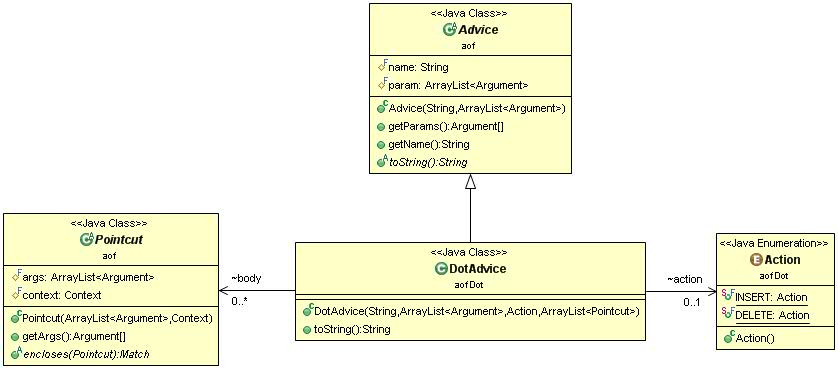
\includegraphics[scale=0.6]{images/AOFDot/DotAdvice.jpg}
\caption{UML diagram of the DotAdvice class.}
\label{fig:DotAdvice}
\end{figure}
\\
TODO: Examples

\section{Order}
Despite the absence of runtime behaviour it is still possible that conflicts arise if two advices modify the same element and the modifications overlap. Just think of an advice that colors a node red, and another that colors it blue. By changing the order of these two advices we either get a red node or a blue one. To specify an order, we simply create a point-comma separated list of the order in which they have to be executed. If there are two advices without an order that do execute at the same time, the order is undetermined.\\
TODO: Example

\section{Weaver}
The weaver will first gather all advices and after that it will start executing them. This is important as it means that if one advice modifies an element in such a way that it no longer matches a pointcut any changes caused by advices liked to that pointcut will still be executed.\\
\\
No other important notes are to be made. Thanks to the Dot compiler it is easy to get all the graphs, nodes and edges from a file modify them and write the resulting graph back to file.\\
\begin{figure}
\centering
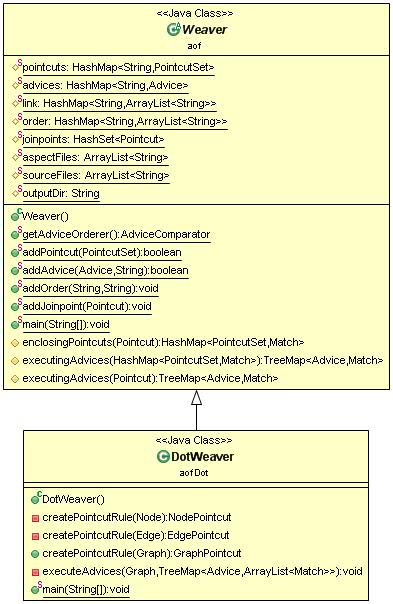
\includegraphics[scale=0.7]{images/AOFDot/DotWeaver.jpg}
\caption{UML diagram of the DotWeaver class.}
\label{fig:DotWeaver}
\end{figure}

\section{Examples}
TODO

\section{Difficulties}
The biggest problem encountered was how to decide on the syntax of the Aspect Orientation Language. Once this was done adding Aspect Orientation went really fast, also thanks to the compiler which allowed it to easily modify the graph and write it back to file.\\
\\
One small problem was that there were two minor bugs in the compiler which needed to be fixed first, but this could be done really fast due to the availability of the source code.

\chapter{AOWP}
AOWP (TODO: REF) is a domain specific language for web applications. Most web applications are developed with the Model-View-Controller framework which clearly separates the application into business logic (model layer) and the visual component (view layer), which communicate through the controller. It is however this framework that makes general AOP languages unfeasible as they break this clear separation.\\
\\
Though there exists an AOP language for PHP called AOPHP, this language has some flaws. First of all there is a lack of pointcuts to really cover all join points of web applications. Secondly there is no way to handle a history of page visits without modifying the web pages. Finally we note that the aspects can not be sufficiently separated from the crosscutting concerns.

\section{Join Point Model}
The join points that can occur in a web application consists of events based on HTTP and language specifications of well-known Web programming languages such as PHP and Java/Servlet. Where the first consists of receiving HTTP requests, reading form data and reading or writing cookie data, the latter consists of reading the session data. An overview of all the events is shown in table (TODO: REF).
\begin{table}
\centering
\begin{tabular}{l|l}
\hline
Abbreviation & Event\\
\hline
\hline
REQ & Receive an HTTP Request\\
\hline
F/R & Read the form data\\
\hline
C/R & Read the cookie data\\
\hline
C/W & Write the cookie data\\
\hline
S/R & Read the session data\\
\hline
S/W & Write the session data\\
\hline
\end{tabular}
\caption{AOWP events}
\label{tab:AOWP_Events}
\end{table}


\section{Aspect Language}
AOWP re-uses the syntax of web programming languages such as PHP and Java/Servlet. It does this by mapping the aspect constructs on to object oriented structures. By doing this the effort required by the user is minimizes as he doesn't need to learn a new language.\\
\\
Creating an aspect can be done by creating a class that extends the Aspect class, adding a pointcut and an advice is done by declaring functions with the name of respectively 'pointcut' and the name of the type of advice ('before', 'after', 'around'). (TODO: example)\\
\\
This could also be accomplished if we were to use the framework, since it is required to create an aspect language of our own. This means that the same syntax could be chosen, though it has to be said that the framework has no notion of aspects, but this is not a problem as it is the responsibility of the compiler to extract the required information and provide it to the weaver in a format it understands.

\section{Pointcuts}
There are three categories of pointcuts, a first one selects events, a second selects event flows and a third selects based on usage contexts. Each of these categories has a set of sub-types, or so called designators. An overview of all the designators are given in tables (TODO: REF).
\begin{table}
\centering
\begin{tabular}{l|p{7cm}}
\hline
Designator & Description\\
\hline
\hline
request & Select REQ with the specified URL\\
\hline
getget & Select specified F/R in a GET request\\
\hline
postget & Select specified F/R in a POST request\\
\hline
cookieget & Select specified C/R\\
\hline
cookieset & Select specified C/W\\
\hline
sessionget & Select specified S/R\\
\hline
sessionset & Select specified S/W\\
\hline
\end{tabular}
\caption{Designators for selecting AOWP events}
\label{tab:Designators_AOWP_Events}
\end{table}
\begin{table}
\centering
\begin{tabular}{l|p{7cm}}
\hline
Designator & Description\\
\hline
\hline
withinrequest & Select all AOWP events in a REQ\\
\hline
pflow & Select all AOWP events in specified page transitions\\
\hline
\end{tabular}
\caption{Designators for selecting AOWP event flows}
\label{tab:Designators_AOWP_Flows}
\end{table}
\begin{table}
\centering
\begin{tabular}{l|p{7cm}}
\hline
Designator & Description\\
\hline
\hline
accessnum & Select all AOWP events when the number of access users is the specified number or greater.\\
\hline
\end{tabular}
\caption{Designators based on usage contexts}
\label{tab:Designators_AOWP_Contexts}
\end{table}
How these designators are used can be seen in table (TODO:REF).
\begin{table}
\centering
\begin{tabular}{l|p{7cm}}
\hline
Example & Description\\
\hline
\hline
request(/news.php) & Selects all events of receiving HTTP requests on news.php.\\
\hline
withinrequest(/login.php) & Selects all events generedted during the execution of HTTP requests for login.php\\
\hline
pflow(/news.php) & Selects all the events involved in handling HTTP requests when the user has seen news.php\\
\hline
accessnum(5) & Selects all events involved in handling HTTP Requests when the number of users if 5 or more.\\
\hline
request(/*Action.php) & Selects the REQ whose name starts with '/' and ends with 'Action.php'.\\
\hline
!pflow(/news.php) & Selects a negative set of events selected by pflow(/news.php)\\
\hline
\end{tabular}
\caption{Designators based on usage contexts}
\label{tab:Designators_AOWP_Contexts}
\end{table}
From this table we also see that it is possible to use regular expressions as an argument of a designator.\\
\\
I will now discuss how these pointcuts could be implemented with the earlier presented framework. Instead of creating a pointcut subclass for each category it is more interesting to only create one subclasses being AOWPPointcut. I choose to take all the pointcuts together as their is no distinction in how these are represented. The class will rely on the arguments of the Pointcut superclass to implement the argument. The specific designator this instance represents has to be indicated by a special value, either an enum or an integer.\\
\\
By doing this we can easily specify pointcuts, creating join points is however a bit more tricky due to capturing the flow. We could do this naivly and create a pointcut for each element along the flow, but that would cause a long delay. It is much better to capture the entire flow as a context and provide that along with the join point. This means that checking whether a pointcut matches a join point is a bit more work, but it allows us to generate only one instance for the entire join point. (TODO: Example)\\
\\
AOWP allows combining multiple designators by using the negation (!), intersection (\&) and union ($|$) operator. This is not possible with the framework, since this only supports union. It is however not a big problems as we can create a new type of pointcut, the OperatorPointcut. This pointcut will simply execute a certain operator (!, \& or $|$) on its members, which are again pointcuts. Another approach could have been to use the union of the framework and using the OperatorPointcut only for the negation and intersection, but this would lead to some extra work to be done. We would have to rework some expressions to make the unions the top-level operator or remote them completely. This can be seen in the following examples. In these examples I use simple letters to represent pointcuts.\\
\begin{align*}
!\left(a | b\right) \& c & \Rightarrow \left(!a \& !b\right) \& c\\
\left(a | b \right) \& !c & \Rightarrow \left(a \& !c\right) | \left(b \& !c \right)
\end{align*}
To avoid this extra work it makes more sense to treat the union the same way as the negation and the intersection.

\section{Advice}
The types of advice AOWP supports is the same as AspectJ, being 'before', 'after' and 'around'. The body of an advice is normal code. Because this is the same as Small C, which is explained earlier, I will not discuss this here again.

\section{Weaver}
Due to the dynamic behaviour of web applications it is impossible to rely on compile time weaving, and thus run-time weaving is required. The weaver itself works pretty straightforward by extracting join point shadows and injects code to call the weaver.\\
\\
This would cause some problems when using the framework, as the current version does not support run-time weaving. A work-around is to set up the weaver each time it is required, but this introduces a large overhead for creating and loading the pointcuts each time.
\section{Examples}
TODO

\chapter{AspectMatlab}
TODO

\chapter{Conspects}
TODO

\chapter{DISL}
TODO

\chapter{KALA}
TODO


\chapter{Discussion}
- To what extent are parts being reused? (or not)\\
- How much coupling is there between the base language and the module?\\
- How flexible is the model? What range of base languages can it handle?
\chapter{Future Work}
- Add the concept of 'Aspects', this will be similar to Objects in an OO language.\\
- Add global variables, is this useful? We will need a general wrapper.\\
- It should be easier to use it on run-time.\\
- Debugging isn't really possible -> keep links from the weaved to the original code.\\
- Optimizing the weaving process, currently each change will require to completely re-weave all the code.\\
\chapter{Related Work}
- About building languages from modules in general .. or about building languages out of smaller languages (also called language composition)
\chapter{Conclusion}

\chapter{Temporary Stuff About Languages}
It is impossible to keep on implementing more and more languages. Therefor I will discuss existing aspect oriented languages and how they could be implemented using the framework.
\section{AOWP}


TODO: REFERENCE!\\
As mentioned in the paper, we need to provide a context to be able to handle coming from a certain page. This can be done by adding this information to the context of the pointcut and join point. The paper mentions different events the language can handle, if the language were to be made with the framework we would have to create a PoincutRule for each of these events (or divide them into groups!).\\
\\
The framework does not provide the '\&' or '!' operator, only the '|' is available by specifying multiple pointcutrules in one poincut. Though it is an inconvience, it is not a big problem since we can create an AndPointcutRule which simply takes two other pointcutrules and matches if both match. The same goes for the NotPointcutRule which will invert the result of a pointcutRule.\\
\\
In it's current form the framework does not provide run-time weaving. It is however to solve this problem in two different ways. The first is by adding extra code that checks the run-time information and makes a decision based on that. The second is by calling the weaver at run time.  By doing this the run-time information is available at the moment of weaving and can be used to specify pointcuts.\\
\\
Since the framework lets the user specify a languages as he likes, the same language can be used as in the paper as long as there is a compiler for it.

\section{AspectMatlab}
TODO: REFERENCE!\\
To add extra information to the pointcuts as is done in the paper, we have to add members to the specific subclasses of the PointcutRule.\\
\\
Pointcuts are: call and execution of methods, get and set of arrays and a special loop pointcut. The within will not be part of the PointcutRule but will be provided as a context.\\
\\
The translation to matlab code can be done the same way with the framework as it was done in the paper.\\
\\
AspectMatlab orders the pointcuts implicitly, the designed framwork does not do this. This means that to maintain the implicit ordering caused by the order of appearance we need to add an explicit ordering to the pointcuts during parsing.\\
\\
The context selectors add contexts to the pointcut or advice (DON'T UNDERSTAND! LOOK IT UP!!!) which can be done by using the context for PointcutRules.\\
\\
The designed framework does not provide a way to share information between advices, or even between the same advices that is run multiple times. To achieve this we have to rely on the options present in the base language. (LOOK UP: is there static stuff in matlab?!)
\section{Conspects}
TODO: REFERENCE!\\
REREAD THIS, it doesn't make much sense!\\
\\
To be able to work with the framework we need to shift a lot of things, first we note that the contexts as presented in the paper can not be achieved. This is however not really a problem since they can be implemented as plain Java Classes.\\
The idea of the event methods that are presented in the paper match what the framework considers a pointcut, there are however some differences. The framework does not allow code in pointcuts in contrary to event methods. The optional guard that can be added will result in a context for the pointcutrule.\\
\\
There seem to be an explicit invocation of events, this can not be done with the framework, and I need to look into this a bit more.\\
There seem to be no real pointcuts, they are part of the advice. This will not be a problem for the framework.
\section{DISL}
The open joinpoint model can be implemented by having a general pointcut to represent a set of byte code instructions. It's up to the parser to detect these sets of byte code.\\
\\
Compatibility with Java and the Java virtual machine is in my opinion achievable since the framework is written in Java. If we look at the more general idea of compatibility we may encounter some problems that are hard to fix and require some workarounds.\\
\\
Access to context data can easily be provided by adding it to the join point and at the same time we can check on this data by setting it in the point cut as a kind of guard. Allowing the user to define its own context elements is harder. How we can do this is not clear, let me think about it.\\
To add the dynamic information it is best to run the weaver at run time.\\
\\
Instrumentations map to advice.\\
Markers map to pointcuts.\\
To add custom markers the weaver needs to be able to detect them, how are we going to do this? Let me think about it.\\
\\
The order is based on numbers: these need to be turned into an partial order, but that's easy.\\
Also, the implicit order of appearance has to be made explicit to the weaver. The parser can do this by making an order while parsing where he states that the previous encountered one must occur before the next encountered.\\
\\
The communication between snippets may be a problem.\\
Static \& Dynamic information: try to hack it in -> We can just do this! (Or what is meant with this?)\\
Guards \& Scope: add context to pointcuts (or part of pointcuts itself). It can be used as a guard if the pointcut has filled in information.
\section{KALA}
TPMonitor => Specify Outside of framework? => Communication?\\
\\
Actions of transaction depend on run-time. (TPMonitor guards this => determines what to do)\\
Secundary transaction: requires check at run-time.\\
\\
KALA declaration = pointcut, no names are used (pointcut needs to have name -> add it while parsing).\\
The extra properties declared inside it are the advice.\\
Framework requires splitting them, but this can be done implicit by the parser.\\
\\
Framework doesn't care about content of advice, that's up to the parser. This makes nested blocks possible.\\
\\
Translating code to work with TPMonitor can be done.\\
Using Reflex will become impossible, but the idea remains the same.\\

\backpages
\begin{appendices}
\chapter{An appendix}
\label{chapt:appendix}

\end{appendices}

%\begin{thebibliography}{9}
%\bibitem{Laddad10}
%  Ramnivas Laddad,
%  \emph{AspectJ In Action}.
%  Manning Publications, Greenwich,
%  2nd Edition,
%  2010
%
%\bibitem{AOWP}
%  
%  Aspect-oriented Programming for Web Controller Layer
%Keiji Hokamura
%Naoyasu Ubayashi
%Shin Nakajima
%Akihito Iwai
%\end{thebibliography}

\end{document}
